\section{Stability of a Rocket}

A rocket in order to fly in a controlled manner has to be stable \cite{web:rocketnasa}. Figure \vref{fig:unstableRocketTrajectory} gives a good example of chaotic trajectory due to unstable design.

\begin{figure} [htbp]
	\centering
	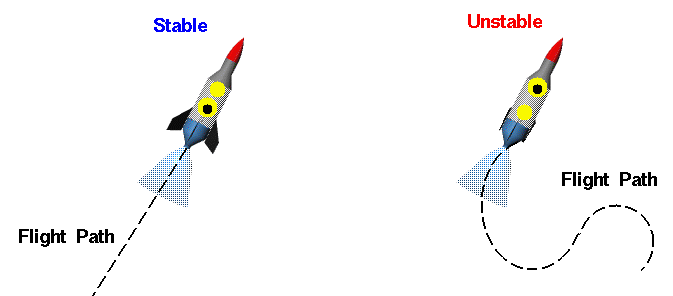
\includegraphics[width=0.4\linewidth]{figures/"Preanalysis&Requirement"/RocketStability/UnstableRocketTrajectory}
	\caption{Example of trajectory for an unstable rocket \cite{web:rocketnasa}.}
	\label{fig:unstableRocketTrajectory}
\end{figure}

To see how a stable rocket has to be designed an analysis of the force applying to the rocket needs to be done. Figure \vref{fig:RocketForceSummary} shows the different situations a rocket encounters during its flight and describes the forces applied in these cases.

\begin{figure} [htbp]
	\centering
	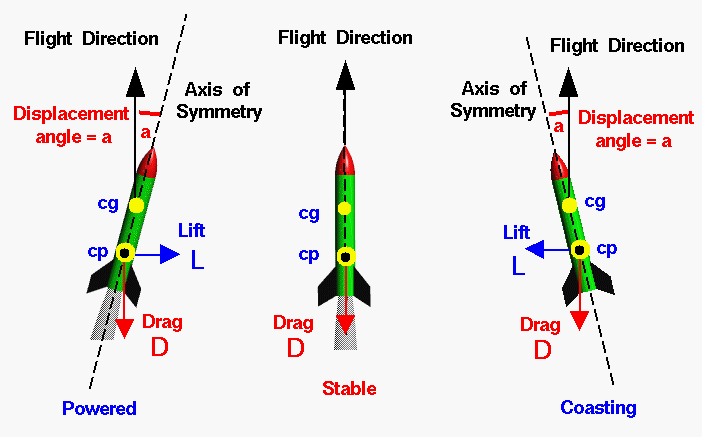
\includegraphics[width=1\linewidth]{figures/"Preanalysis&Requirement"/RocketStability/ForceSummaryRocket}
	\caption{Summary of forces applied to a rocket during its flight \cite{web:rocketnasa}.}
	\label{fig:RocketForceSummary}
\end{figure}

In figure \vref{fig:RocketForceSummary} two points can be seen on the rockets. The first one CP Center of Pressure is where the  lift and the drag force apply \cite{web:rocketnasa}. The second one is CG Center of Gravity, it is the point where the rocket rotate \cite{web:rocketnasa}. Due to this characteristics the torque applied by the lift and the drag is dependent of the relative positioning between the CG and the CP. Since a rocket tilts due to a torque applied by external forces such as the wind, the lift and the drag has to be oriented so it counters these forces. In order to do so the CP has to be above the CG \cite{web:rocketnasa}.
This means depending of the position of the CP compared to the CG the rocket flight will be either stable or unstable.

However there might be case where the construction can only be unstable such as actual full scale rocket. In this case a control system has to be designed, in order to counter the torques applied by the external forces reinforced by the drag and the lift.